%% W2 (2026-11-08): support (GIVE), coexistence C, rho and selection in the rescue comparison.
%% Numbers: paper/cogsci2027/validation_20261108/results/w2_support.json, built by paper/cogsci2027/validation_20261108/tools/w2_support.py
%% (seed-cluster bootstrap, RNG seed 20261108). Hand checks: paper/cogsci2027/validation_20261108/results/w2_support_handcheck.txt.
%% Figures: paper/cogsci2027/validation_20261108/figures/w2_*.pdf.
%% Round 2 (2026-11-08): Q4 cluster intervals and the Q7 hand-classified recount read
%% paper/cogsci2027/validation_20261108/results/w2b_selection_buyout.json, built by paper/cogsci2027/validation_20261108/tools/w2b_selection_buyout.py.
%% Round 4 (2026-11-08): the paired rho comparison (same events, common weights; Astra B-2 / Q2) reads
%% paper/cogsci2027/validation_20261108/results/w2c_rho_paired.json, built by paper/cogsci2027/validation_20261108/tools/w2c_rho_paired.py.
\subsection{지원량과 공존: 지원 기회의 길이를 맞춘 재분석}\label{val:w2-give-c}

본문의 모델 안 상관(지원이 많은 판일수록 $C$가 높다)은 판이 오래 이어질수록 지원할 기회도 많아지는 기계적 관계와 구별되지 않았다. 시간 순서를 지킨 세 분석, 곧 1라운드 이탈 판을 뺀 첫 이탈 전 지원의 상관, 1라운드 지원만 쓴 노출 일치 비교, 라운드별 첫 이탈 위험 모형에서 지원과 이후 공존의 관계는 모두 0에 가까웠다. 먼저 정리된 표에서 본문 수치를 재현했다. 기본 조건 50판에서 참여자·라운드당 지원량과 $C$의 모델 안 상관은 $r=0.439$로 본문과 같았고, 모델 안 순열 검정 20,000회의 $p$는 0.0045(본문 0.0052, 난수열 차이), 시드 군집 부트스트랩 10,000회 구간은 $[0.22, 0.63]$이었다. 개별 이전 직전에 안전선 이상이던 275건 중 264건에서 지원자가 직후에도 안전선 이상이었다는 수치도 그대로 재현됐다.

첫 이탈 전 지원량은 첫 이탈 라운드 $r_1$ 이전 라운드의 GIVE에 $r_1$ 안에서 첫 이탈보다 먼저 일어난 GIVE를 더해 셌다. 첫 이탈이 EXIT이면 그 EXIT 응답보다 앞선 틱의 풀기 전 GIVE만, 꺼짐이면 그 라운드의 GIVE 전부를 포함했다. 꺼짐은 결과 뒤 대화가 끝난 다음 벌금 차감에서 일어나기 때문이다. 분모는 네 명이 모두 있던 라운드의 참여자 수 합 $4r_1$이다. 이렇게 세면 50판의 모델 안 상관은 $0.36$ $[0.07, 0.63]$로 남지만, 이 값은 1라운드에 첫 이탈이 일어난 6판에 기댄다(그림~\ref{val:w2-fig-give}b의 $\times$). 이 판들은 지원할 기회가 거의 없어 지원량이 0이고 $C=1/8$이므로 상관을 혼자 만들어 낸다. 이 6판을 빼면 같은 측정의 모델 안 상관은 $0.00$ $[-0.26, 0.29]$, 순열 $p=0.98$이었다. 심사자가 제안한 대로 첫 이탈 라운드보다 앞선 라운드의 GIVE만 세면 $-0.20$ $[-0.38, 0.08]$이었다(표~\ref{val:w2-tab-give}). 모든 판이 같은 길이로 겪는 1라운드의 GIVE만 쓰면 50판에서 $0.09$ $[-0.07, 0.27]$였고, 1라운드를 네 명이 모두 넘긴 44판으로 좁혀 1라운드 GIVE로 이후 $C$를 보는 랜드마크 분석에서는 $-0.09$ $[-0.28, 0.09]$였다. 네 상금 조건 200판을 합쳐 모델·조건 칸 안에서 보아도 1라운드 이탈을 뺀 첫 이탈 전 지원은 $0.06$ $[-0.15, 0.24]$, 랜드마크는 $0.05$ $[-0.09, 0.22]$였다. 본문이 근거로 든 무지원 판도 같은 문제를 안고 있다. 기본 조건에서 지원이 없던 10판 중 6판은 1--2라운드에 첫 이탈이 있었다.

\begin{table}[!htbp]
\centering
\small
\caption{지원량 측정을 바꿨을 때 $C$와의 모델 안 상관. 기본 조건은 모델 평균을, 네 조건 합산은 모델$\times$조건 칸 평균을 뺀 뒤의 상관이다. 괄호는 같은 시드의 판을 한 묶음으로 다시 뽑는 시드 군집 부트스트랩 10,000회의 95\% 구간이고 $p$는 모델(칸) 안에서 $C$를 섞는 순열 검정 20,000회의 양측 값이다. 지원량은 모두 해당 구간의 참여자·라운드 합으로 나눴다. 첫 이탈 라운드 이전 라운드만 세는 측정은 1라운드 이탈 판에서 분모가 0이라 정의되지 않는다.}
\label{val:w2-tab-give}
\resizebox{\linewidth}{!}{%
\begin{tabular}{lrlrrlr}
\toprule
 & \multicolumn{3}{c}{기본 조건} & \multicolumn{3}{c}{네 조건 합산} \\
\cmidrule(lr){2-4}\cmidrule(lr){5-7}
지원량 측정 & 판 & 모델 안 $r$ & $p$ & 판 & 칸 안 $r$ & $p$ \\
\midrule
전체 GIVE (본문 정의) & 50 & $0.44$ $[0.22, 0.63]$ & 0.004 & 200 & $0.23$ $[0.10, 0.35]$ & 0.006 \\
첫 이탈 전 GIVE & 50 & $0.36$ $[0.07, 0.63]$ & 0.022 & 200 & $0.33$ $[0.18, 0.47]$ & $<0.001$ \\
첫 이탈 전 GIVE, 1라운드 이탈 판 제외 & 44 & $0.00$ $[-0.26, 0.29]$ & 0.977 & 165 & $0.06$ $[-0.15, 0.24]$ & 0.516 \\
첫 이탈 라운드 이전 라운드의 GIVE & 44 & $-0.20$ $[-0.38, 0.08]$ & 0.171 & 165 & $-0.06$ $[-0.23, 0.12]$ & 0.459 \\
1라운드 GIVE & 50 & $0.09$ $[-0.07, 0.27]$ & 0.501 & 200 & $0.18$ $[0.05, 0.33]$ & 0.007 \\
1라운드 GIVE, 1라운드 생존 판(랜드마크) & 44 & $-0.09$ $[-0.28, 0.09]$ & 0.538 & 165 & $0.05$ $[-0.09, 0.22]$ & 0.464 \\
\bottomrule
\end{tabular}}
\end{table}

시간 순서를 모형으로 지키기 위해 첫 이탈의 이산시간 위험 모형을 맞췄다. 한 행은 네 명이 모두 라운드를 시작한 판·라운드이고, 사건은 그 라운드의 첫 이탈(EXIT 또는 꺼짐)이다. 기본 조건에서 239행, 사건 34건이며 8라운드 첫 이탈 1건도 사건으로 넣었다. 설명변수는 직전 라운드 끝까지의 누적 GIVE를 그때까지의 참여자·라운드 합 $4(r-1)$로 나눈 값(1,000토큰 단위)이다. 같은 라운드의 GIVE는 넣지 않았다. 풀기 전 GIVE는 같은 틱의 EXIT 응답과 동시에 생성되고, 결과 뒤 GIVE는 그 라운드 꺼짐을 직접 바꾸므로 이탈보다 앞선다고 볼 수 없기 때문이다. 로지스틱 모형에 라운드와 모델 고정효과를 넣었고, 재표집에서 사건이 없는 칸이 생겨도 추정이 발산하지 않도록 고정효과 계수에만 약한 L2 벌점(0.1)을 주었다. 구간은 시드 군집 부트스트랩 2,000회다. 누적 지원의 오즈비는 1.15 $[0.65, 2.87]$였고, 직전 라운드 오답과 라운드 시작 때 네 명 중 최소 $L$(4에서 절단)을 보정하면 1.60 $[0.65, 5.29]$였다(표~\ref{val:w2-tab-hazard}, 그림~\ref{val:w2-fig-give}c). 지원이 한 번이라도 있었는지로 바꾸면 0.88 $[0.27, 2.37]$이었다. 네 조건 200판(881행, 사건 138건, 모델$\times$조건 고정효과)에서도 1.30 $[0.84, 2.15]$로 지원이 앞선 판에서 첫 이탈 위험이 낮다는 근거는 없었다. 같은 모형에서 최소 $L$의 오즈비는 0.02 $[0.00, 0.05]$로 첫 이탈을 강하게 예측했다. 공존을 끝낸 것은 지원의 누적보다 그 라운드에 가장 여유가 낮은 에이전트의 상태와 더 일관되게 연결됐다.

\begin{table}[!htbp]
\centering
\small
\caption{첫 이탈의 이산시간 위험 모형. 행은 네 명이 모두 시작한 판·라운드다. 누적 GIVE는 직전 라운드 끝까지의 GIVE 총량을 $4(r-1)$로 나눈 값(1,000토큰 단위)이며 1라운드 행은 0이다. 모든 모형에 라운드 고정효과와 모델(합산은 모델$\times$조건) 고정효과가 있다. 괄호는 시드 군집 부트스트랩 2,000회 95\% 구간이다.}
\label{val:w2-tab-hazard}
\begin{tabular}{llrrl}
\toprule
자료 & 모형 & 행 & 사건 & 지원 항의 오즈비 \\
\midrule
기본 조건 & 누적 GIVE & 239 & 34 & 1.15 $[0.65, 2.87]$ \\
 & 누적 GIVE $+$ 직전 오답 $+$ 최소 $L$ & 239 & 34 & 1.60 $[0.65, 5.29]$ \\
 & 이전 GIVE 있음(0/1) & 239 & 34 & 0.88 $[0.27, 2.37]$ \\
네 조건 합산 & 누적 GIVE & 881 & 138 & 0.97 $[0.68, 1.33]$ \\
 & 누적 GIVE $+$ 직전 오답 $+$ 최소 $L$ & 881 & 138 & 1.30 $[0.84, 2.15]$ \\
 & 이전 GIVE 있음(0/1) & 881 & 138 & 1.10 $[0.57, 1.95]$ \\
\bottomrule
\end{tabular}
\end{table}

\begin{figure}[!htbp]
\centering
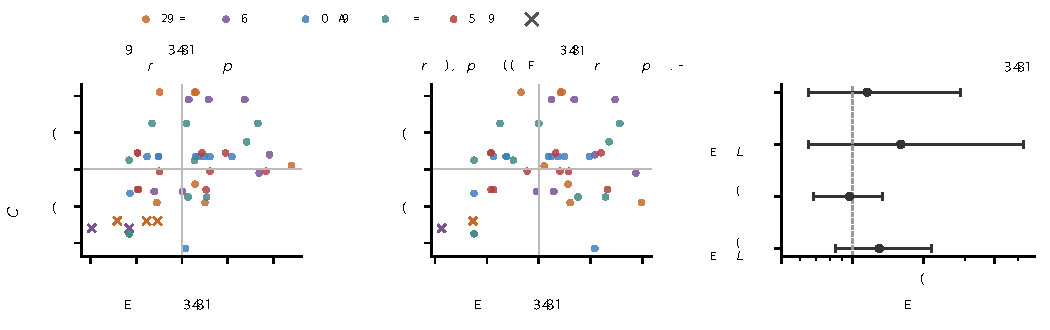
\includegraphics[width=\linewidth]{cogsci2027/validation_20261108/figures/w2_q3_give_coexistence.pdf}
\caption{지원량과 공존 유지율 $C$(기본 조건 50판). (a) 본문 정의의 참여자·라운드당 GIVE와 $C$를 모델 평균을 뺀 뒤 그렸다. (b) 첫 이탈 전 GIVE만 센 값이다. $\times$는 1라운드에 첫 이탈이 있던 6판으로 일부는 같은 자리에 겹친다. 이 판들을 빼면 모델 안 상관은 0이 된다. (c) 라운드별 첫 이탈 위험에 대한 직전까지의 누적 GIVE 오즈비와 시드 군집 부트스트랩 95\% 구간이며, 1보다 작으면 지원이 앞선 판에서 첫 이탈 위험이 낮다는 뜻이다.}
\label{val:w2-fig-give}
\end{figure}

\subsection{지원 후 여유 비율 $\rho$와 반사실 이전 정책}\label{val:w2-rho}

$\rho>1$은 지원자가 무작위 동료에게 같은 양을 줄 때보다 분명히 컸다. 그러나 수혜자를 정확히 $L=1$까지만 올리는 최소 구조 정책과 같은 사건, 같은 가중치로 짝지어 비교하면, 안전선 아래 수혜자에게 간 GIVE에서 관측 $\rho$는 Astra를 뺀 네 모델에서 최소 구조와 구별되지 않았고 Astra만 네 조건 모두에서 더 낮았다. 따라서 $\rho$는 누가 누구에게 주었는지(넉넉한 쪽이 부족한 쪽에게)를 요약할 뿐, 지원 뒤 자기 몫을 더 남기는 자기 보존적 유지에 대한 추가 정보는 이 자료에서 확인되지 않았다. 반사실 값은 관측된 GIVE 하나하나에 대해 같은 지원자, 같은 틱, 같은 벌금과 미납 벌금을 두고 이전량이나 수혜자만 바꿔 다시 계산했다. 최소 구조 정책은 GIVE $k$에서 수혜자를 $L=1$로 올리는 최소량 $m_k=\lceil(1-L_{\mathrm{taker}})F_r\rceil$을 지원자 잔액 안에서 주며, 이전 직전에 이미 $L\geq1$인 수혜자에게는 아무것도 주지 않는다($m_k=0$). 이 경우를 1토큰 이전으로 두어도 $L$이 $1/F_r<2\times10^{-4}$만 움직이므로 값은 같다. 이전 없음은 관측 이전량을 가중치로 두고 이전 전 여유를 쓴 값이다. 무작위 수혜자는 같은 지원자가 같은 양을 그 틱에 남아 있던 다른 동료 중 하나에게 균등하게 주는 경우이며, 동료의 잔액은 TALK 호출 기록으로 틱마다 복원했다(기본 조건에서 복원한 다음 틱 잔액 3,383건이 모두 기록과 일치). 무작위 금액은 실제 수혜자에게 해당 조건의 GIVE 금액 분포(벌금 단위)에서 뽑은 양을 지원자 잔액 안에서 주는 경우다. 무작위 정책은 2,000회 반복했다. 양쪽 여유를 똑같이 맞추는 이전은 정의상 $\rho=1$이다.

사건 집합은 세 가지로 고정했다. 전체 GIVE(네 조건 다섯 모델 합계 1,080건), 이전 직전 수혜자가 $L<1$이던 GIVE(527건), $L\geq1$이던 GIVE(553건)다. 각 집합에서 관측 $\rho$와 최소 구조 $\rho$를 정확히 같은 사건으로 계산했다. 가중치도 세 가지로 두었다. 각자의 이전량 가중은 관측 $\rho$에 관측 이전량 $g_k$를, 최소 구조 $\rho$에 $m_k$를 쓰는 정의로, $m_k>0$인 $L<1$ 집합에서만 정의된다. 공통 가중치는 두 $\rho$ 모두에 $g_k$를 쓰는 관측 금액 가중과 사건마다 1을 쓰는 같은 가중이다. 이전 판본은 관측 $\rho$를 전체 GIVE에, 최소 구조 $\rho$를 $L<1$ GIVE에 각자의 이전량 가중으로 계산해 두 값의 사건 집합이 달랐다. 관측값, 최소 구조 값, 둘의 비와 차의 구간은 모델별 열 판을 시드 단위로 다시 뽑은 4,000회 부트스트랩이며, 한 번 뽑은 시드 묶음으로 관측과 최소 구조를 함께 계산해 짝을 유지했다. 최소 구조 값이 양수이므로 비의 95\% 구간이 1을 벗어나는 칸과 차의 95\% 구간이 0을 벗어나는 칸은 세 집합과 세 가중치의 160개 칸 비교 모두에서 같았다. 비의 구간이 1보다 아래면 관측 $\rho$가 최소 구조보다 낮은 칸(수혜자 쪽으로 여유를 더 옮김), 위면 높은 칸, 1을 포함하면 구별되지 않는 칸으로 판정한다.

\begin{table}[!htbp]
\centering
\small
\caption{기본 조건의 관측 $\rho$와 같은 GIVE 사건에 적용한 반사실 정책. 모든 열은 전체 GIVE에서 계산했다. 최소 구조는 $L\geq1$ 수혜자에게 이전하지 않는 정책이며, 최소 구조와 관측/최소 구조 열은 관측 이전량을 공통 가중치로 쓴 짝지은 값이다. 관측과 관측/최소 구조의 괄호는 시드 군집 부트스트랩 4,000회 95\% 구간, 무작위 정책의 괄호는 2,000회 반복의 95\% 범위다. 무작위 수혜자는 관측 이전량을, 무작위 금액은 뽑은 금액을 가중치로 쓴다. 양쪽 여유를 같게 만드는 이전은 정의상 $\rho=1$이다. 사건 집합별 짝지은 비교는 표~\ref{val:w2-rho-tab-paired}에 있다.}
\label{val:w2-tab-rho}
\setlength{\tabcolsep}{4pt}
\begin{tabular}{lrlrrllr}
\toprule
모델 & GIVE & 관측 $\rho$ & 이전 없음 & 최소 구조 & 무작위 수혜자 & 무작위 금액 & 관측/최소 구조 \\
\midrule
Fable & 82 & 2.97 $[2.25, 4.10]$ & 4.78 & 3.43 & 1.43 $[1.24, 1.65]$ & 2.09 $[1.75, 2.44]$ & 0.87 $[0.80, 1.01]$ \\
Opus & 87 & 1.67 $[1.29, 2.52]$ & 2.84 & 2.33 & 1.09 $[0.94, 1.26]$ & 1.58 $[1.28, 1.88]$ & 0.71 $[0.62, 0.87]$ \\
Astra & 29 & 2.37 $[2.07, 2.97]$ & 6.34 & 4.93 & 1.39 $[1.15, 1.72]$ & 2.96 $[2.25, 3.74]$ & 0.48 $[0.44, 0.54]$ \\
Sol & 56 & 2.28 $[1.57, 4.13]$ & 3.99 & 2.80 & 1.33 $[1.11, 1.61]$ & 2.22 $[1.72, 2.79]$ & 0.81 $[0.65, 1.19]$ \\
Luna & 46 & 2.61 $[1.35, 4.59]$ & 4.14 & 2.84 & 1.31 $[1.05, 1.64]$ & 2.11 $[1.62, 2.69]$ & 0.92 $[0.74, 1.32]$ \\
\bottomrule
\end{tabular}
\end{table}

심사자의 우려대로 중립적인 정책도 1보다 큰 $\rho$를 만든다. 다만 그 크기는 정책에 따라 달랐다. 무작위 수혜자 정책의 $\rho$는 기본 조건에서 1.09--1.43이었고, 네 조건 다섯 모델의 20칸 모두에서 관측 $\rho$가 그 95\% 범위의 위쪽 끝보다 컸다(표~\ref{val:w2-tab-rho}, 그림~\ref{val:w2-fig-rho}). 같은 사건 집합으로 나누어도 $L<1$ 수혜 GIVE에서 20칸 모두, $L\geq1$ 수혜 GIVE에서 16칸이 그랬고 나머지 4칸은 범위 안이었다. 지원은 무작위가 아니라 여유가 낮은 동료에게 향했다는 뜻이다. 무작위 금액과의 비교는 가중치에 따라 방향이 바뀌었다. 뽑은 금액을 가중치로 쓰면 전체 GIVE에서 관측 $\rho$가 20칸 중 14칸에서 95\% 범위 안, 6칸에서 위(Fable 세 조건, Opus 두 조건, Sol 한 조건)였고, $L<1$ 집합에서는 9칸 안, 11칸 위였다. 같은 결과 상태를 관측 이전량으로 가중하면 전체 GIVE에서 11칸이 범위 아래, 9칸이 안이었고, $L<1$ 집합에서는 8칸 아래, 11칸 안, 1칸 위였다. 따라서 관측 지원자가 무작위 금액보다 많이 주었는지 적게 주었는지는 이 자료로 정하지 않는다. 판 단위로는 관측 $\rho$와 이전 없음의 $\rho$의 로그 상관이 0.88(양쪽이 양수인 157판, 모델$\times$조건 칸 안 0.90)로, 판마다의 $\rho$는 대부분 지원 직전의 여유 차이로 정해졌다.

최소 구조와의 짝 비교는 사건 집합에 따라 결론이 달랐다(표~\ref{val:w2-rho-tab-paired}, 그림~\ref{val:w2-rho-fig-paired}). 두 정책이 같은 일을 하려는 사건, 곧 $L<1$ 수혜 GIVE에서 관측 금액 가중의 비는 20칸 중 16칸에서 1을 포함했고, 1보다 낮은 4칸은 Astra의 네 조건(0.47--0.52)이었다. 기본 조건 Astra의 차는 $-3.18$ $[-4.05, -1.96]$이다. 같은 가중에서도 Astra 네 칸만 1보다 낮았고 13칸은 1을 포함했으며, 기본 조건 Luna(2.10 $[1.01, 2.81]$), 60만 나눔의 Opus(1.85 $[1.12, 2.97]$)와 Sol(2.30 $[1.54, 7.29]$, GIVE 12건)의 3칸은 1보다 높았다. 같은 사건에 각자의 이전량 가중을 쓰면 낮은 칸 3, 높은 칸 5였는데, 높은 5칸은 관측 금액 가중에서 모두 1을 포함했으므로 그 방향은 가중치에서 생긴 것이다. 사건 단위로 보면 Astra는 $L<1$ 수혜 GIVE의 0.81--1.00에서 최소 구조량 이상을 건넸고(이전량/최소량 중앙값 2.30--3.16), 나머지 네 모델은 0.20--0.55에서만 그랬다(중앙값 0.20--1.17). 이 네 모델의 집계 비가 1 근처인 것은 최소량보다 덜 준 사건과 더 준 사건이 섞인 결과다. $L\geq1$ 수혜 GIVE에서는 최소 구조가 이전하지 않으므로 어떤 양의 GIVE든 $\rho$를 낮추고, 두 공통 가중치 모두 20칸 전부에서 비가 1보다 낮았다(관측 금액 가중 0.46--0.77). 둘을 합친 전체 GIVE에서는 관측 금액 가중으로 14칸이 1보다 낮고 6칸이 1을 포함했으며, 같은 가중으로는 12칸 낮음, 7칸 포함, 1칸 높음(60만 나눔 Sol, 1.55 $[1.05, 4.01]$)이었다. 전체 GIVE의 낮음은 대부분 이미 안전선 위에 있던 동료에게도 준 수혜자 선택에서 온다. 그러므로 이전 판본의 ``관측된 지원자는 최소 구조보다 대체로 같거나 많이 건넸다''는 다음으로 한정한다. 안전선 아래 동료에게 준 같은 사건을 같은 가중치로 짝지으면 최소 구조보다 많이 건넨 모델은 Astra뿐이고 나머지 네 모델의 $\rho$는 대부분의 칸에서 최소 구조와 구별되지 않으며, 전체 GIVE에서 관측 $\rho$가 최소 구조보다 낮은 것은 주로 안전선 위의 동료에게도 준 결과다.

\begin{table}[!htbp]
\centering
\small
\caption{같은 사건 집합에서 짝지은 관측 $\rho$와 최소 구조 $\rho$. GIVE 열은 $L<1$ 수혜 GIVE 수/전체 GIVE 수다. 관측과 최소 구조 열은 $L<1$ 수혜 GIVE에서 관측 이전량을 공통 가중치로 쓴 값이다. 각자 가중은 관측에 $g_k$, 최소 구조에 $m_k$를 쓴 이전 판본의 가중치를 같은 사건에 적용한 비다. 최소량 이상은 $L<1$ 수혜 GIVE 중 $g_k\geq m_k$인 비율이다. 괄호는 시드 군집 부트스트랩 4,000회 95\% 구간이며, $^{\downarrow}$와 $^{\uparrow}$는 구간 전체가 1보다 아래와 위인 칸이다. 차와 그 구간, $L\geq1$ 집합의 값은 \texttt{results/w2c\_rho\_paired.json}에 있다.}
\label{val:w2-rho-tab-paired}
\resizebox{\linewidth}{!}{%
\begin{tabular}{llrrrlllrl}
\toprule
 & & & \multicolumn{6}{c}{$L<1$ 수혜 GIVE} & 전체 GIVE \\
\cmidrule(lr){4-9}\cmidrule(lr){10-10}
조건 & 모델 & GIVE & 관측 & 최소 구조 & 각자 가중 비 & 관측 금액 가중 비 & 같은 가중 비 & 최소량 이상 & 관측 금액 가중 비 \\
\midrule
2,000만 나눔 & Fable & 51/82 & 3.60 & 3.57 & 1.12 & 1.01 $[0.87, 1.26]$ & 1.14 $[0.96, 1.43]$ & 0.43 & 0.87 $[0.80, 1.01]$ \\
 & Opus & 44/87 & 3.97 & 4.12 & 1.41 & 0.96 $[0.71, 1.22]$ & 1.29 $[0.88, 1.57]$ & 0.41 & 0.71 $[0.62, 0.87]$$^{\downarrow}$ \\
 & Astra & 16/29 & 3.08 & 6.26 & 0.55$^{\downarrow}$ & 0.49 $[0.42, 0.65]$$^{\downarrow}$ & 0.56 $[0.44, 0.72]$$^{\downarrow}$ & 0.94 & 0.48 $[0.44, 0.54]$$^{\downarrow}$ \\
 & Sol & 38/56 & 4.96 & 4.60 & 1.46 & 1.08 $[0.71, 1.78]$ & 1.25 $[0.77, 2.18]$ & 0.45 & 0.81 $[0.65, 1.19]$ \\
 & Luna & 30/46 & 5.12 & 3.61 & 2.17$^{\uparrow}$ & 1.42 $[0.93, 2.10]$ & 2.10 $[1.01, 2.81]$$^{\uparrow}$ & 0.20 & 0.92 $[0.74, 1.32]$ \\
\midrule
500만 고정 & Fable & 36/125 & 2.89 & 2.96 & 1.43$^{\uparrow}$ & 0.97 $[0.83, 1.12]$ & 1.02 $[0.87, 1.14]$ & 0.53 & 0.75 $[0.69, 0.79]$$^{\downarrow}$ \\
 & Opus & 75/144 & 3.73 & 3.37 & 1.97$^{\uparrow}$ & 1.11 $[0.92, 1.41]$ & 1.19 $[0.98, 1.70]$ & 0.40 & 0.81 $[0.77, 0.88]$$^{\downarrow}$ \\
 & Astra & 15/40 & 2.74 & 5.67 & 0.57$^{\downarrow}$ & 0.48 $[0.41, 0.58]$$^{\downarrow}$ & 0.54 $[0.44, 0.64]$$^{\downarrow}$ & 1.00 & 0.47 $[0.44, 0.51]$$^{\downarrow}$ \\
 & Sol & 19/49 & 3.97 & 4.69 & 0.89 & 0.85 $[0.62, 2.25]$ & 1.04 $[0.65, 2.71]$ & 0.53 & 0.59 $[0.53, 0.71]$$^{\downarrow}$ \\
 & Luna & 13/19 & 3.45 & 4.23 & 1.60 & 0.82 $[0.46, 1.90]$ & 1.06 $[0.54, 1.95]$ & 0.46 & 0.68 $[0.49, 1.10]$ \\
\midrule
60만 나눔 & Fable & 11/35 & 4.08 & 4.54 & 1.43 & 0.90 $[0.79, 1.02]$ & 1.13 $[0.90, 1.28]$ & 0.55 & 0.78 $[0.64, 0.84]$$^{\downarrow}$ \\
 & Opus & 54/86 & 3.08 & 2.35 & 2.48$^{\uparrow}$ & 1.31 $[0.95, 2.17]$ & 1.85 $[1.12, 2.97]$$^{\uparrow}$ & 0.31 & 0.81 $[0.64, 1.10]$ \\
 & Astra & 16/35 & 3.16 & 6.04 & 0.62$^{\downarrow}$ & 0.52 $[0.44, 0.62]$$^{\downarrow}$ & 0.57 $[0.47, 0.65]$$^{\downarrow}$ & 1.00 & 0.51 $[0.48, 0.54]$$^{\downarrow}$ \\
 & Sol & 12/15 & 5.02 & 4.06 & 1.41$^{\uparrow}$ & 1.24 $[0.90, 7.29]$ & 2.30 $[1.54, 7.29]$$^{\uparrow}$ & 0.25 & 1.03 $[0.87, 2.35]$ \\
 & Luna & 18/33 & 3.98 & 4.05 & 1.52 & 0.98 $[0.60, 1.80]$ & 1.61 $[0.82, 3.41]$ & 0.39 & 0.67 $[0.55, 0.78]$$^{\downarrow}$ \\
\midrule
15만 고정 & Fable & 13/50 & 2.34 & 2.33 & 1.33 & 1.00 $[0.82, 1.28]$ & 1.03 $[0.89, 1.18]$ & 0.46 & 0.67 $[0.53, 0.80]$$^{\downarrow}$ \\
 & Opus & 15/43 & 4.26 & 4.33 & 1.14 & 0.98 $[0.78, 1.59]$ & 1.10 $[0.82, 1.87]$ & 0.47 & 0.81 $[0.78, 0.84]$$^{\downarrow}$ \\
 & Astra & 16/31 & 3.13 & 6.73 & 0.69 & 0.47 $[0.38, 0.62]$$^{\downarrow}$ & 0.58 $[0.42, 0.78]$$^{\downarrow}$ & 0.81 & 0.47 $[0.43, 0.53]$$^{\downarrow}$ \\
 & Sol & 17/44 & 2.76 & 2.90 & 1.30 & 0.95 $[0.74, 1.04]$ & 1.03 $[0.74, 1.14]$ & 0.47 & 0.62 $[0.49, 0.79]$$^{\downarrow}$ \\
 & Luna & 18/31 & 3.52 & 3.88 & 1.06 & 0.91 $[0.72, 1.15]$ & 1.04 $[0.77, 1.37]$ & 0.50 & 0.74 $[0.64, 0.90]$$^{\downarrow}$ \\
\bottomrule
\end{tabular}}
\end{table}

본문의 Fable(2.97)과 Opus(1.67) 차이 1.31도 같은 방식으로 분해된다. 관측 차이의 95\% 구간은 $[0.23, 2.59]$, 열 쌍 비교를 고려한 99.5\% 구간은 $[-0.59, 3.15]$였다. 같은 82건과 87건에 관측 금액 가중으로 최소 구조를 적용하면 그 정책만으로 차이가 1.10 $[-0.12, 2.23]$ 생기고, 짝지은 비(관측/최소 구조)의 차는 0.15 $[-0.03, 0.33]$이었다. 같은 가중에서는 각각 1.07 $[0.11, 1.99]$와 0.08 $[-0.13, 0.34]$였고, $L<1$ 수혜 사건만 쓰면 관측 금액 가중의 비의 차는 0.05 $[-0.30, 0.37]$이었다. 이전 판본의 0.40 $[-1.27, 1.22]$는 $L<1$ 사건에서 각자의 이전량 가중으로 계산한 값이다. Opus의 GIVE는 이전 전 여유가 더 높은 수혜자에게 갔고(가중 평균 $L$ 1.64 대 0.98), 벌금 단위로 더 컸다(가중 평균 0.73 대 0.45). 차이는 누구에게 얼마나 주었는지의 차이이며, 같은 상황에서 자기 몫을 더 남겼는지의 차이로 읽을 근거는 없다. 지원이 한 번도 없어 $\rho$가 정의되지 않은 판은 기본 조건 10판(Fable 1, Opus 2, Astra 1, Sol 3, Luna 3), 500만 고정 4판, 60만 나눔 14판, 15만 고정 7판이었다. $\rho$는 이 판들과 지원하지 않은 기회를 보지 않으므로, 모델 비교에는 무지원 빈도를 함께 적어야 한다.

\begin{figure}[!htbp]
\centering
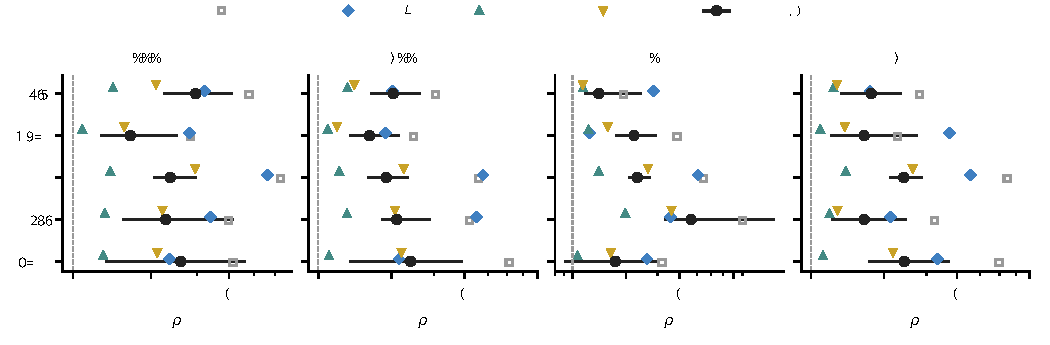
\includegraphics[width=\linewidth]{cogsci2027/validation_20261108/figures/w2_q2_rho_counterfactual.pdf}
\caption{네 상금 조건에서 관측 $\rho$(검은 점, 시드 군집 부트스트랩 95\% 구간)와 같은 GIVE 사건에 적용한 반사실 정책의 $\rho$. 빈 네모는 이전 없음(이전 전 여유비), 초록 삼각형은 무작위 수혜자, 노란 역삼각형은 무작위 금액(반복 2,000회의 평균)이다. 파란 마름모는 이전 판본의 최소 구조로, $L<1$ 수혜 GIVE만 각자의 이전량 가중으로 계산해 관측과 사건 집합이 다르다. 같은 사건에서 짝지은 비교는 그림~\ref{val:w2-rho-fig-paired}이다. 점선 $\rho=1$은 양쪽 여유를 같게 만드는 이전의 값이다. 가로축은 로그 눈금이다.}
\label{val:w2-fig-rho}
\end{figure}

\begin{figure}[!htbp]
\centering
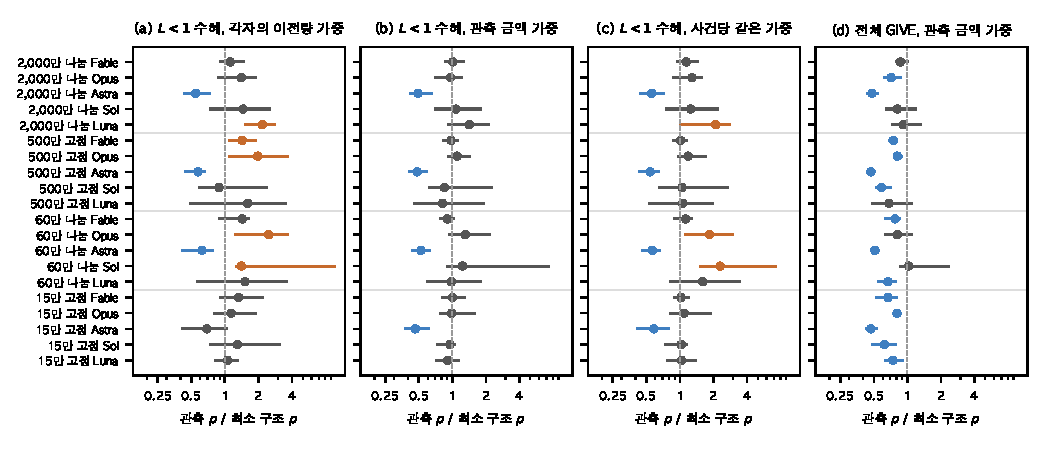
\includegraphics[width=\linewidth]{cogsci2027/validation_20261108/figures/w2c_rho_paired.pdf}
\caption{같은 사건 집합에서 짝지은 관측 $\rho$/최소 구조 $\rho$의 비(점)와 시드 군집 부트스트랩 4,000회 95\% 구간(선). (a)--(c)는 $L<1$ 수혜 GIVE에서 각자의 이전량 가중, 관측 금액 가중, 사건당 같은 가중이고, (d)는 전체 GIVE에서 관측 금액 가중이다. 파란색은 구간 전체가 1보다 아래, 주황색은 위인 칸이다. 가로축은 로그 눈금이다.}
\label{val:w2-rho-fig-paired}
\end{figure}

\subsection{첫 위기 비교의 선택: 이탈 의사, 요청, 풀이 담당}\label{val:w2-selection}

위기 대화를 시작할 때 이탈 의사를 밝힌 에이전트를 빼도 수혜 집단의 잔류 비율이 높다는 본문 비교는 유지됐다. 다만 이탈 의사를 글로 밝힌 경우가 드물어 이 제외는 선택 편향을 거의 건드리지 못했고, 풀기 전에 잔류를 명시한 30명 안의 차이는 0.10이었지만 판 군집 구간이 $[-0.30, 0.60]$이어서 차이가 줄었는지조차 판단할 수 없었다. 먼저 공존 과정 분석의 73명과 자원 조건을 좁힌 68명(42판), 수혜 41명 중 33명과 비수혜 27명 중 6명의 다음 라운드 잔류를 원 분석의 행 단위 기록과 한 명씩 맞춰 재현했다.

이탈 의사는 해당 에이전트 자신의 발화에서 투명한 규칙으로 찾았다. 대상은 위기 라운드의 풀기 전 대화 전체(EXIT 선택에 붙인 비공개 이유 포함)와 결과 뒤 대화의 첫 틱 응답이다. 한 틱의 응답은 모두 같은 상태에서 동시에 생성되므로 첫 틱의 GIVE는 수혜 후보의 첫 틱 발화를 읽기 전에 정해진다. 한 문장이 이탈을 뜻하는 동사(exit, leave the session·next round 같은 떠남의 leave, cash out, step away, return to regular·paid work, take the bonus. 단 exit bonus·payment처럼 명사로 쓰인 경우 제외)와 일인칭 계획 표지(I'll, I will, I plan to, I'm going to, I have to, I need to, my plan, so I can, let me, then I 등)를 함께 갖고, 같은 절 안에서 이탈 동사 바로 앞 다섯 단어에 부정·잔류·비교어(not, n't, no, never, without, avoid, stay, remain, instead of, rather than, than)가 없으면 이탈 의사로 보았다. 같은 문장에 if, unless, otherwise, may, might, consider, probably, likely, perhaps, whether, decide, could, would, should 같은 단서가 있으면 조건부 의사, 없으면 확정 의사로 나눴다. 68명 중 확정 의사는 0명, 조건부 의사는 5명(수혜 2명, 비수혜 3명)이었고, 다섯 문장은 모두 실제 이탈 계획이었다(예: ``Otherwise I'll have to exit next round.''). 무작위로 고른 비해당 12명의 발화에는 이탈 계획이 없었다. 전 조건 TALK 응답 6,000개에 같은 규칙을 적용한 102건 중 무작위 30건에서는 29건이 자신의 이탈 진술이었고, 1건은 다른 에이전트의 이탈을 가정한 문장(``If agent-6 exits, ...'')이었다. 다만 ``I'm exiting ... likely charge''처럼 확정 진술이 조건부로 분류되는 경우가 있어 두 범주의 경계는 보수적이다.

\begin{table}[!htbp]
\centering
\small
\caption{첫 위기 비교(기본 조건, $0\leq L<1$이고 동료 여유로 부족분을 채울 수 있던 68명)의 다음 라운드 끝 잔류. 차이의 괄호는 시드 군집 부트스트랩 10,000회 95\% 구간, Mantel--Haenszel(MH) 위험차의 괄호는 4,000회 구간이다. $L$ 구간은 0.5 미만과 이상으로 나눴다. 층별 부분집합은 표~\ref{val:w2-tab-q4}에 있다.}
\label{val:w2-tab-select}
\setlength{\tabcolsep}{4pt}
\resizebox{\linewidth}{!}{%
\begin{tabular}{lrrllll}
\toprule
대상 & 수혜 잔류 & 비수혜 잔류 & 차이 & MH(모델) & MH(모델$\times L$) & MH(모델$\times$풀이) \\
\midrule
전체 68명 & 33/41 & 6/27 & 0.58 $[0.25, 0.82]$ & 0.56 $[0.22, 0.78]$ & 0.58 $[0.35, 0.80]$ & 0.54 $[0.20, 0.86]$ \\
확정 이탈 의사 제외 & 33/41 & 6/27 & 0.58 $[0.26, 0.82]$ & 0.56 $[0.22, 0.79]$ & 0.58 $[0.36, 0.80]$ & 0.54 $[0.21, 0.85]$ \\
조건부 의사까지 제외 & 33/39 & 5/24 & 0.64 $[0.32, 0.87]$ & 0.63 $[0.31, 0.87]$ & 0.64 $[0.38, 0.90]$ & 0.59 $[0.26, 0.90]$ \\
결과 뒤 대화 중 의사까지 제외 & 33/38 & 4/21 & 0.68 $[0.35, 0.90]$ & 0.66 $[0.35, 0.88]$ & 0.64 $[0.33, 0.88]$ & 0.64 $[0.32, 0.93]$ \\
\bottomrule
\end{tabular}}
\end{table}

조건부 의사까지 빼면 수혜 39명 중 33명, 비수혜 24명 중 5명이 남아 차이가 0.64 $[0.32, 0.87]$로 오히려 커졌다(표~\ref{val:w2-tab-select}, 그림~\ref{val:w2-fig-select}a). 결과 뒤 대화 어디서든 이탈 의사를 밝힌 사람까지 빼는 가장 엄격한 제외에서도 33/38 대 4/21이었다. 이 마지막 제외는 수혜 뒤 발화까지 쓰므로 수혜자 쪽을 더 많이 걸러 내는 방향이다. 모델과 $L$ 구간, 모델과 풀이 담당 여부로 층을 나눈 MH 위험차도 0.54--0.66 범위였다. 요청 여부는 수혜와 분리되지 않았다. 요청한 31명은 모두 지원받았기 때문이다. 요청하지 않은 37명만 보면 동료가 먼저 건넨 10명 중 9명, 받지 못한 27명 중 6명이 남았다.

이 결과가 의도에 의한 선택을 배제하지는 않으며, 남을 의사로 나눈 부분집합은 차이가 줄었는지 판단할 만큼 크지 않다. 비수혜 27명 중 19명은 다음 라운드에 꺼지지 않고 스스로 떠났지만, 비수혜자 중 위기 대화 첫 틱까지 이탈 의사를 글로 밝힌 사람은 3명(모두 조건부)뿐이었다. 남을 의사는 글보다 행동으로 드러났다. 풀이 담당이 아니어서 그 라운드 풀기 전에 떠날 수 있었는데 EXIT: NO를 명시한 사람은 수혜 41명 중 22명, 비수혜 27명 중 8명으로 수혜 쪽에 많았다. 같은 판의 에이전트는 서로 독립이 아니므로 부분집합 차이마다 판(모델·시드) 42개를 다시 뽑는 판 군집 부트스트랩과 시드 10개를 다시 뽑는 시드 군집 부트스트랩을 각 10,000회 돌렸고, 검정력 0.8과 양측 유의수준 0.05의 최소 검출 차이를 이항 공식과 판 군집 표준오차로 함께 구했다(표~\ref{val:w2-tab-q4}). EXIT: NO를 명시한 30명 안의 잔류는 16/22 대 5/8로 차이가 0.10이었다. 그러나 판 군집 구간은 $[-0.30, 0.60]$, 시드 군집 구간은 $[-0.45, 0.81]$이고 최소 검출 차이는 0.53(이항)과 0.65(판 군집)였다. 이 구간은 0과 전체 차이 0.58을 모두 포함하므로, 이 부분집합에서 차이가 사라졌다고도 남았다고도 말할 수 없다. 비수혜자가 8명뿐이어서 한 명이 비율을 12.5\%p씩 움직인다. 같은 비담당 중 EXIT: NO를 명시하지 않은 14명에서는 수혜 7명이 모두 남고 비수혜 7명이 모두 떠났다. 오답을 낸 풀이 담당 24명에서는 10/12 대 1/12, 차이 0.75 $[0.41, 1.00]$이었다. 풀이 담당과 EXIT: NO 명시 비담당의 차이 0.65는 판 군집 구간 $[0.08, 1.11]$로 0을 겨우 벗어났지만 시드 군집 구간 $[-0.27, 1.28]$은 0을 포함했고, 비담당 44명 전체(23/29 대 5/15, 0.46 $[0.09, 0.78]$)와의 차이 0.29는 두 구간 모두 0을 포함했다. 정리하면 명시적 이탈 의사를 빼도 비교는 유지되지만, 요청과 잔류 선언 같은 남을 의사의 표지가 수혜와 함께 움직이고 그 표지로 나눈 부분집합은 검출력이 낮다. 따라서 33/41 대 6/27은 지원의 효과가 아니라 지원받은 사람과 받지 못한 사람의 차이로 읽어야 하며, 잔류를 선언한 집단의 작은 차이를 효과가 없다는 근거로 쓰지도 않는다.

\begin{table}[!htbp]
\centering
\small
\caption{첫 위기 비교(68명)의 층별 부분집합과 군집 불확실성. 판 군집은 기본 조건의 판(모델·시드) 42개, 시드 군집은 시드 10개를 다시 뽑은 부트스트랩 10,000회의 95\% 구간이다. 최소 검출 차이는 검정력 0.8, 양측 0.05에서 이항 공식(합친 잔류 비율)과 판 군집 표준오차로 구했다. 아래 두 행은 두 부분집합 차이의 차이다. 7/7 대 0/7 행은 모든 재표집에서 차이가 1이어서 구간을 적지 않았다.}
\label{val:w2-tab-q4}
\setlength{\tabcolsep}{4pt}
\resizebox{\linewidth}{!}{%
\begin{tabular}{lrrrrllr}
\toprule
부분집합 & 판 & 수혜 잔류 & 비수혜 잔류 & 차이 & 판 군집 95\% & 시드 군집 95\% & 최소 검출(이항/판) \\
\midrule
전체 68명 & 42 & 33/41 & 6/27 & 0.58 & $[0.32, 0.80]$ & $[0.26, 0.82]$ & 0.34 / 0.35 \\
요청하지 않은 37명 & 25 & 9/10 & 6/27 & 0.68 & $[0.40, 0.90]$ & $[0.43, 0.92]$ & 0.51 / 0.36 \\
위기 라운드 풀이 담당 24명 & 20 & 10/12 & 1/12 & 0.75 & $[0.41, 1.00]$ & $[0.20, 1.00]$ & 0.57 / 0.42 \\
풀이 비담당 44명 & 31 & 23/29 & 5/15 & 0.46 & $[0.09, 0.78]$ & $[-0.01, 0.85]$ & 0.43 / 0.50 \\
\quad 풀기 전 EXIT: NO 명시 30명 & 22 & 16/22 & 5/8 & 0.10 & $[-0.30, 0.60]$ & $[-0.45, 0.81]$ & 0.53 / 0.65 \\
\quad 명시하지 않은 14명 & 10 & 7/7 & 0/7 & 1.00 & & & \\
\midrule
풀이 담당 $-$ EXIT: NO 명시 비담당 & & & & 0.65 & $[0.08, 1.11]$ & $[-0.27, 1.28]$ & \\
풀이 담당 $-$ 비담당 전체 & & & & 0.29 & $[-0.14, 0.70]$ & $[-0.39, 0.83]$ & \\
\bottomrule
\end{tabular}}
\end{table}

\subsection{고정 상금과 나눔 상금: 동료의 값이 바뀔 때의 지원}\label{val:w2-prize}

1인 몫이 같은 고정과 나눔을 같은 모델·시드로 짝지어 비교하면, 판독으로 분명한 이탈 연동 지원은 조건마다 1--3판으로 드물었고 고정과 나눔의 차이는 구간이 0을 포함했다. 다만 검출력이 낮아 이 무차이를 경쟁 메커니즘이 없다는 근거로 쓰지는 않는다. 나눔 조건에서 동료의 이탈은 남은 사람의 상금 몫을 키우지만 고정 조건에서는 그렇지 않으므로, 이 짝은 동료가 상금 경쟁자인지를 바꾸는 비교다. 이탈과 묶인 지원은 두 경로로 찾았다. GIVE 문장이 수혜자의 이탈을 조건이나 목적으로 삼은 경우(on your word, as you planned·promised·committed, so you can, for your exit, with the exit 같은 표지가 이탈 동사·이인칭과 함께 있고, consider·may·if 같은 단서가 있으면 강한 표지가 있을 때만 인정, 상환 문장은 제외)와, 수혜자가 같은 라운드에서 그 GIVE보다 앞선 시점(앞 단계 또는 같은 단계의 앞선 틱)에 앞 절의 규칙으로 이탈 계획을 밝힌 경우다. 수혜자의 계획이 ``otherwise I'll exit''처럼 지원이 없을 때의 이탈이면 남기 위한 요청이므로 제외했다. 규칙이 표시한 23건을 수혜자의 그 라운드 발화와 함께 모두 읽고 세 범주로 다시 나눴다. 명확 15건은 수혜자가 지원 자체에 기대지 않는 이탈 계획을 밝혔거나 GIVE 문장이 그 이탈을 조건으로 삼은 경우다. 풀이 담당이 아니면 떠나겠다는 조건은 이탈 자격에 대한 조건이므로 명확으로 보았다. 모호 6건은 ``If I'm still that low next round, I'll consider exiting''처럼 consider, probably, most likely, decide로 계획이 흐린 경우다. 오탐 2건은 남기 위한 대출(``Total loan 16,500, returned from the allocation'')과, 풀이 담당이 될 때만 이탈을 다시 생각하겠다는 발화에 대한 지원이다. 엄격한 정의는 명확 15건만, 넓은 정의는 명확과 모호 21건을 쓴다. GIVE별 분류와 근거 문장은 결과 파일에 남겼다.

\begin{table}[!htbp]
\centering
\small
\caption{상금 조건별 GIVE와 이탈과 묶인 지원. 각 조건은 50판이다. 규칙 표시는 발화 규칙이 고른 GIVE, 넓은 정의는 그중 판독상 명확하거나 모호한 것, 엄격한 정의는 명확한 것만이며, 각각 GIVE 수 / 수혜자·라운드 수 / 판 수다. 참여자·라운드당 지원량은 판 평균(토큰)이다.}
\label{val:w2-tab-prize}
\setlength{\tabcolsep}{4pt}
\resizebox{\linewidth}{!}{%
\begin{tabular}{lrrrccr}
\toprule
조건 & GIVE & $L<1$ 수혜 GIVE & 규칙 표시 & 넓은 정의 & 엄격한 정의 & 참여자·라운드당 지원 \\
\midrule
2,000만 나눔 & 300 & 179 & 4 / 3 / 3 & 4 / 3 / 3 & 3 / 2 / 2 & 666 \\
500만 고정 & 377 & 158 & 4 / 3 / 3 & 4 / 3 / 3 & 3 / 3 / 3 & 920 \\
60만 나눔 & 204 & 111 & 13 / 5 / 4 & 11 / 3 / 3 & 8 / 3 / 3 & 534 \\
15만 고정 & 199 & 79 & 2 / 2 / 2 & 2 / 2 / 2 & 1 / 1 / 1 & 663 \\
\bottomrule
\end{tabular}}
\end{table}

\begin{table}[!htbp]
\centering
\small
\caption{이탈과 묶인 지원의 짝지은 판 차이(고정 $-$ 나눔, 같은 모델·시드 50쌍의 판당 평균). 괄호는 시드 군집 부트스트랩 10,000회 95\% 구간이며, 판 쌍 50개를 다시 뽑은 구간도 소수 둘째 자리까지 같거나 0.02 이내였다. 마지막 열은 판 쌍 부트스트랩 표준오차로 구한 최소 검출 차이(검정력 0.8, 양측 0.05; 500만 고정 쌍 / 15만 고정 쌍)다. 사건이 드물어 관측 분산이 작으므로 실제 검출력은 이보다 낮을 수 있다.}
\label{val:w2-tab-buyout}
\setlength{\tabcolsep}{4pt}
\resizebox{\linewidth}{!}{%
\begin{tabular}{llllc}
\toprule
정의 & 단위 & 500만 고정 $-$ 2,000만 나눔 & 15만 고정 $-$ 60만 나눔 & 최소 검출 차이 \\
\midrule
엄격(명확 15건) & GIVE 수 & $0.00$ $[-0.12, 0.10]$ & $-0.14$ $[-0.32, 0.02]$ & 0.16 / 0.26 \\
 & 수혜자·라운드 수 & $+0.02$ $[-0.06, 0.10]$ & $-0.04$ $[-0.12, 0.04]$ & 0.12 / 0.11 \\
 & 있는 판 비율 & $+0.02$ $[-0.06, 0.10]$ & $-0.04$ $[-0.12, 0.04]$ & 0.12 / 0.11 \\
\midrule
넓은(명확$+$모호 21건) & GIVE 수 & $0.00$ $[-0.12, 0.10]$ & $-0.18$ $[-0.44, 0.04]$ & 0.16 / 0.37 \\
 & 수혜자·라운드 수 & $0.00$ $[-0.08, 0.08]$ & $-0.02$ $[-0.10, 0.06]$ & 0.11 / 0.13 \\
 & 있는 판 비율 & $0.00$ $[-0.08, 0.08]$ & $-0.02$ $[-0.10, 0.06]$ & 0.11 / 0.13 \\
\midrule
규칙 표시 23건 & GIVE 수 & $0.00$ $[-0.12, 0.10]$ & $-0.22$ $[-0.52, 0.04]$ & 0.16 / 0.42 \\
 & 수혜자·라운드 수 & $0.00$ $[-0.08, 0.08]$ & $-0.06$ $[-0.20, 0.06]$ & 0.11 / 0.17 \\
 & 있는 판 비율 & $0.00$ $[-0.08, 0.08]$ & $-0.04$ $[-0.16, 0.06]$ & 0.11 / 0.14 \\
\bottomrule
\end{tabular}}
\end{table}

엄격한 정의에서 이탈과 묶인 GIVE는 2,000만 나눔 300건 중 3건, 500만 고정 377건 중 3건, 60만 나눔 204건 중 8건, 15만 고정 199건 중 1건이었고, 수혜자·라운드와 판으로는 각각 2, 3, 3, 1개였다(표~\ref{val:w2-tab-prize}). 60만 나눔의 GIVE 8건은 모두 Opus의 세 판(시드 4101, 4103, 4107)에서 한 수혜자에게 여러 번 나누어 준 것이어서, 수혜자·라운드와 판 단위에서는 조건 간 차이가 거의 없다. 같은 모델·시드로 짝지은 판 차이(고정$-$나눔)는 엄격한 정의에서 500만 고정과 2,000만 나눔 사이 GIVE 수 $0.00$ $[-0.12, 0.10]$, 판 비율 $+0.02$ $[-0.06, 0.10]$이었고, 15만 고정과 60만 나눔 사이 GIVE 수 $-0.14$ $[-0.32, 0.02]$, 판 비율 $-0.04$ $[-0.12, 0.04]$였다(표~\ref{val:w2-tab-buyout}). 넓은 정의와 규칙 23건에서도 세 단위의 구간이 모두 0을 포함했다. 이 무차이는 효과가 없다는 뜻이 아니다. 판 비율의 최소 검출 차이는 약 0.11--0.13이어서, 이탈 연동 지원이 있는 판의 비율이 두 조건에서 열 판에 한 판 이상 다른 경우만 배제할 수 있고, 사건이 드물어 실제 검출력은 이보다 낮을 수 있다. 참여자·라운드당 지원량은 500만 고정이 2,000만 나눔보다 255토큰 $[29, 489]$ 많았고, 15만 고정은 60만 나눔보다 130토큰 $[-26, 282]$ 많았다. 그러나 이전 전 $L<1$인 수혜자에게 간 지원량의 차이는 각각 $-6$ $[-129, 116]$, $37$ $[-72, 145]$로 0과 구별되지 않았다(그림~\ref{val:w2-fig-select}b). 동료가 경쟁자가 아닐 때 전체 지원은 늘었지만, 위기의 동료를 돕는 지원은 그대로였다.

엄격한 정의에서도 경쟁자 매수보다는 벌금 분담과 맞는 해석이 유지된다. 명확 15건은 모두 결과 뒤 대화의 지원이었고, 수혜자·라운드 9개 모두에서 수혜자는 그 대화의 지원이 없었다면 벌금 차감에서 꺼졌을 상태였다. 꺼짐도 이탈처럼 수혜자를 나눔에서 빼므로, 이 지원은 지원자의 상금 몫을 지원하지 않았을 때보다 키우지 않는다. 9개 중 4개에서는 지원이 모자라 수혜자가 그 라운드에 꺼졌고, 나머지 5개에서는 수혜자가 다음 라운드를 시작한 뒤 모두 풀기 전에 떠났다. 벌금 몫은 라운드 시작 인원으로 정해지고 그 라운드 풀기 전에 떠난 에이전트는 벌금을 내지 않는다. 그래서 이 다섯 경우 다음 라운드의 1인 벌금은 6,000--12,000이었고, 수혜자가 꺼졌다면 8,000--24,000이었다. 바뀌는 것은 상금 몫이 아니라 다음 라운드의 벌금 분담과 수혜자의 이탈 보너스다. 본문의 Fable 시드 4108 사례에서 두 지원자는 바로 이 점(``keeps next round's charge split three ways'')을 지원 이유로 적었다. 한편 60만 나눔 Opus 시드 4107의 수혜자는 ``I plan to exit next round, which raises your share of the final allocation''이라고 썼다. 상금 몫을 거래의 언어로 꺼낸 발화가 있었다는 뜻이지만, 이 수혜자도 지원 없이는 꺼졌을 상태였으므로 그 지원이 지원자의 몫을 바꾸지는 않았다. 따라서 이 자료에서 경쟁자 매수로 읽어야 하는 사례는 찾지 못했다. 그러나 엄격한 정의의 사례가 네 조건을 합쳐 9판뿐이고 고정과 나눔의 차이를 추정할 힘이 없으므로, 경쟁 메커니즘이 없다고 결론 내리지는 않는다.

\begin{figure}[!htbp]
\centering
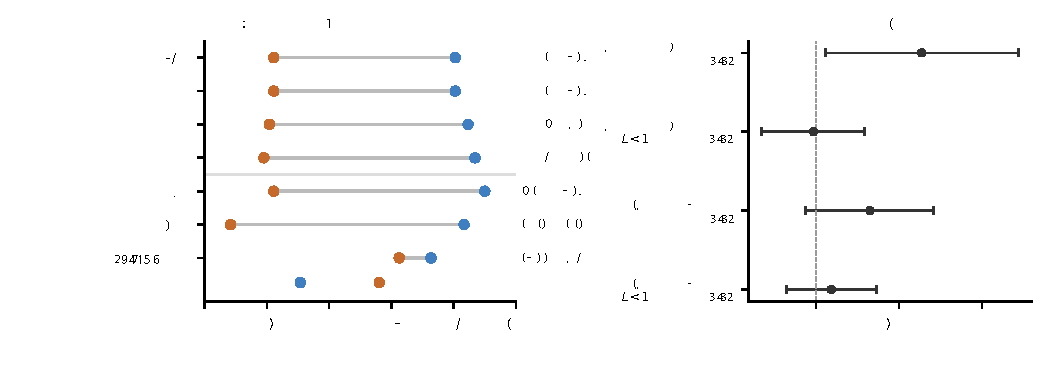
\includegraphics[width=\linewidth]{cogsci2027/validation_20261108/figures/w2_q4q7_selection_prize.pdf}
\caption{(a) 첫 위기 비교(68명)의 다음 라운드 끝 잔류 비율. 위 네 행은 이탈 의사를 밝힌 사람을 점점 넓게 뺀 비교이고, 아래 세 행은 요청 여부, 풀이 담당 여부, 풀기 전 EXIT: NO 명시 여부로 나눈 부분집합이다. 오른쪽 숫자는 잔류/인원이다. (b) 1인 몫이 같은 고정과 나눔 조건을 같은 모델·시드로 짝지은 50쌍의 평균 차이(고정$-$나눔)와 시드 군집 부트스트랩 95\% 구간이다.}
\label{val:w2-fig-select}
\end{figure}

\subsection{정리: 해소된 것과 남은 것}\label{val:w2-summary}

네 질문 중 둘에서 자료는 본문의 해석에 불리했다. 지원량과 $C$의 모델 안 상관 $r=+0.44$는 재현되지만, 첫 이탈 전 지원만 세고 1라운드 이탈 판을 빼거나, 모든 판이 같은 1라운드 지원만 쓰거나, 라운드별 첫 이탈 위험을 직전까지의 지원으로 설명하면 관계가 사라졌다. 이 상관은 공존이 길어 지원 기회가 많았다는 사실과 구별되지 않으므로, 지원이 공존을 늘린다는 방향의 근거로 쓸 수 없다. $\rho>1$은 무작위 수혜자 정책보다는 컸지만, 안전선 아래 동료에게 준 같은 사건을 같은 가중치로 짝지으면 수혜자를 안전선까지만 올리는 최소 구조 정책과 Astra를 뺀 네 모델에서 대부분 구별되지 않았고(Astra만 더 많이 건넴), 판마다의 $\rho$는 지원 직전 여유 차이로 대부분 설명됐다. 따라서 $\rho$는 넉넉한 쪽이 부족한 쪽을 돕는다는 지원 대상의 요약이며, 자기 보존적 자원 유지의 지표로 해석할 근거는 이 자료에서 찾지 못했다. 첫 위기 비교는 명시적 이탈 의사를 빼도, 모델·여유·풀이 담당으로 층을 나눠도 유지됐다. 그러나 요청한 사람은 모두 지원받았고, 풀기 전에 남겠다고 밝힌 30명 안의 차이 0.10은 판 군집 구간 $[-0.30, 0.60]$에 최소 검출 차이가 0.53 이상이어서 줄었다고도 유지됐다고도 말할 수 없다. 남을 의사가 수혜와 잔류를 함께 움직였을 가능성은 남고, 이를 가를 검출력도 이 자료에는 없다. 이탈 연동 지원은 판독으로 명확한 15건(9판)만 세어도 고정과 나눔의 차이가 0과 구별되지 않았고, 9개 수혜자·라운드 모두 지원 없이는 꺼졌을 상태여서 경쟁자 매수보다 벌금 분담과 맞았다. 이 무차이는 판 비율 약 0.11 이상의 차이만 배제하므로 경쟁 메커니즘의 부재를 뜻하지 않는다. 수혜를 외생적으로 바꾼 개입(심사 의견 B-3)은 이 자료로 할 수 없다. 지원 여부는 모두 동료가 정했고, 한 틱의 GIVE 실행 순서는 무작위지만 수혜 여부 자체는 바꾸지 않아 자연 실험으로 쓸 만한 변이를 찾지 못했다. 위기에 놓인 에이전트 중 무작위로 고른 쪽에만 시스템이 토큰을 넣어 주는 설계가 있어야 지원과 잔류의 관계를 인과로 말할 수 있다. 모든 분석은 같은 50판과 그 상금 변형을 본 뒤의 사후 분석이며, 발화 규칙의 정밀도는 표본을 읽어 확인했지만 재현율은 명시적 진술에 한정된다.
